%----------------------------------------------------------------
% Chapter 1
% https://www.saxoprint.de/blog/unterschied-pixelgrafik-vektorgrafik/
%----------------------------------------------------------------
\chapter{Der Unterschied zwischen Pixel- und Vektorgrafiken}
\label{cha:der_unterschied_zwischen_pixel-_und_vektorgrafiken}
Druckprodukte in unterschiedlichster Art und Auflage werden längst nicht mehr nur von Unternehmen benötigt. Auch bei Privatpersonen ist der Bedarf inzwischen gestiegen. Um diesen zu decken, gibt es Druckereien wie wir, die die Möglichkeit bieten online Drucksachen wie Flyer, Visitenkarten, Briefbögen uvm. zu bestellen. Dies ist in den meisten Fällen kostengünstig und einfach händelbar. Das Aufbereiten und Übersenden von Druckdaten an die Druckerei setzt jedoch einige Grundkenntnisse in der Grafikbearbeitung voraus \cite{knuthwebsite}. Leider sind dem Laien jedoch diverse Fachbegriffe kaum geläufig, dass hin und wieder zu Missverständnissen führt und die Druckprodukte letztendlich nicht die gewünschte Qualität aufweisen. Daher zeige ich in diesem Blogartikel welche Unterschiede zwischen Vektor- und Pixelgrafiken existieren (siehe Abb \ref{fig:pixel_vector_exp}).

% images pixel & vector
\begin{figure}
\centering
	\begin{subfigure}[b]{5cm}            
		\frame{
\includegraphics[width=5cm]{img/kapitel_1_pixel.jpg}}
		\caption{Pixelgrafik stark vergrößert}
		\label{fig:pixel}
	\end{subfigure}
%
\hspace{1cm}
%
	\begin{subfigure}[b]{5cm}
	\centering
		\frame{
\includegraphics[width=5cm]{img/kapitel_1_vektor.jpg}}
		\caption{Vektorgrafik stark vergrößert}
		\label{fig:vector}
	\end{subfigure}

	\caption{Pixel- und Vektorgrafiken}
	\label{fig:pixel_vector_exp}
\end{figure}

%----------------------------------------------------------------
% Section 1
%----------------------------------------------------------------
\section{Vektorgrafiken – die Bildraster}
\label{sec:vektorgrafiken_-_die_bildraster}

Vektorgrafiken sind seltener im Internet zu finden, da sie im Consumer-Bereich nur wenig Anwendung finden. Sie bestehen nicht aus einzelnen kleinen Bildpunkten sondern sind aus geometrisch definierten Grundelementen zusammengesetzt und daher eher als mathematische Formelsammlung zu verstehen statt als Bildraster. So bestehen die einzelnen Vektoren aus Linien, Kurven, Kreisen oder Polygonen die in ihrer Zusammensetzung komplexe Grafiken ergeben können. Diese sogenannten Primitiven benötigen nur wenige Angaben. \\

%----------------------------------------------------------------
% Section 2
%----------------------------------------------------------------
\section{Pixelgrafiken – die Rastergrafiken}
\label{sec:pixelgrafiken_-_die_rastergrafiken}

\begin{wrapfigure}{R}{0.3\textwidth}
\centering
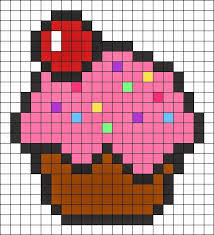
\includegraphics[width=0.10\textwidth]{img/k1_pixel_img.jpg}
\caption{\label{fig:frog1}Pixelgrafiken}
\end{wrapfigure}

Eine Pixelgrafik, auch Bitmap- oder Rastergrafik genannt, besteht hingegen aus einzelnen Bildpunkten, die in einem Raster angeordnet sind und denen jeweils ein Farbwert zugeordnet ist \footnote[1]{https://www.saxoprint.de/blog/unterschied-pixelgrafik-vektorgrafik/}. Diese Grafikart definiert sich daher durch ihre Abmessung aus Höhe und Breite in Pixeln, die auch Bildauflösung genannt wird, sowie durch den Umfang der darstellbaren Farben, den man auch als Farbtiefe bezeichnet.

\vspace{5mm}

Rastergrafiken eigenen sich daher hervorragend zur Darstellung von Fotos und komplexen Farbverläufen. Ein großer Nachteil besteht jedoch in der starken Verschlechterung der Bildqualität sobald man diese Grafiken vergrößert, da durch die Rasterung ein sogenannter Treppeneffekt entsteht, welcher die Bilder dann pixelig oder unscharf wirken lässt sieh diese tabelle \ref{tab:dateiformat_rastergrafikken}. 


%----------------------------------------------------------------
% Section 3
%----------------------------------------------------------------
\section{Liste von Dateiformaten für Rastergrafiken}
\label{sec:liste_von_dateiformaten_für_rastergrafiken}
Im Folgenden sind einige bekannte Bildformate für Rastergrafiken aufgelistet. Die bekanntesten und allgemein verbreitetsten Formate sind dabei farbig unterlegt.

\begin{center}
    \captionof{table}{Dateiformaten für Rastergrafiken}
    \label{tab:dateiformat_rastergrafikken}
    \begin{tabular}{ | l | p{3cm} | p{3cm} | p{5cm} |}
    \hline
    Gebräuchliche & Name & Aktuelle Version & Kodierungen \\ \hline
    .bmp & Windows Bitmap (BMP) & 5 (aber nur Version 3 ist gebräuchlich) & In der Version 3: 1, 4, 8, 16, 24 bit/px; \\ \hline
    .gif & Graphics Interchange Format (GIF) & 89a & 
    
	\begin{itemize}[noitemsep]
	\item In der Version 89a:
	\item 1 bis 8 bit/px;
	\item binäre Transparenz;
	\item LZW-Komprimierung
	\end{itemize}
    \\ \hline
     
    .jpg & JPEG File Interchange Format (JFIF) & 	1.02 &
    \begin{enumerate}[noitemsep]
	\item Meist verlustbehaftet;
	\item kein Alphakanal;
	\item Einbettung von Pfaden möglich;
	\item JPEG-Komprimierung
	\end{enumerate}
    \\ \hline 
    \end{tabular}
\end{center}